We humans are surrounded by lots of items. Those items might be very important or might not be important at all. With having to interact with lots of items it is pretty hard for us to remember what items are needed and where it is located.\\
Pocket-self is the inventory tracking app that helps people to store and record the items that are important in a organized manner. With the help of the app users will be able to record the items in the database and later on retrieve it when needed. Users will be able to choose the particular self or the location that he/she wants to store the item. Then the app helps to enter the location and the item and saves the information in the database. Users will also be able to scan the item rather than having to enter the information manually. So, when the user needs the specific item then he can just search the app and it will tell where exactly is the item located.


\subsection{Purpose and Use}
The purpose of the app is to make the life of user easier by organizing all the items as inventory in an organized fashion. The main goal of app is to store the information of the app in database and retrieve quickly when needed. When the user defines the location of the storage and provides the information about the item that they want to store, then the user can retrieve the information in the future just by doing the quick search. The app will also provide notification about the expiry date and vital information about the product in timely manner. Basically the app is used for storing items information and retrieve the location and information quickly when needed.

\subsection{Intended Audience}
This app is specifically intended for the people who want to organize the items that they have in their houses but, it can also be used for business to record the inventory if needed. This app is more useful for collectors. As for the collectors they have numerous amount of same type of the item. For example, the user might have collection of beverages or books. So, what he can do is he can enter the information and the location of where all the items he wants to store. Then, in future he can retrieve the item with ease.


\begin{figure}[hbt!]
	\centering
   	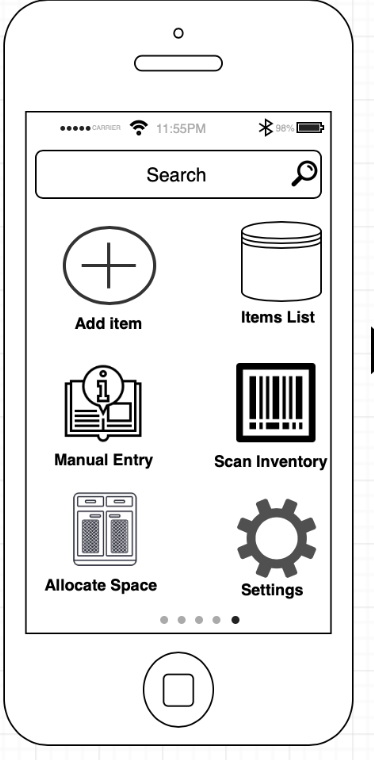
\includegraphics[width=0.60\textwidth]{images/product.PNG}
    \caption{Basic UI of the application}
\end{figure}
